\documentclass[11pt]{article}

\usepackage{nmrdoc}
\usepackage{siunitx}
\usepackage{bm}
\usepackage{tikz}

\sisetup{per-mode=symbol}
\DeclareSIUnit{\angstrom}{\text{\AA}}

\newcommand{\code}[1]{\texttt{#1}}
\setlength{\parindent}{0pt}
\setlength{\parskip}{0.42em}
\emergencystretch=2em

\begin{document}
\NmrTitle{Numerical Addendum: HBond Calculator}

HBond is the McConnell dyadic family evaluated on DSSP-resolved hydrogen-bond
sources. The shared McConnell addendum treats the three-term asymmetric tensor,
the scalar \(f\), the symmetric-traceless dipolar helper, and the
\(T_0/T_1/T_2\) projection; this addendum records what changes here: the source
list comes from DSSP partner slots, the source point is the \(N\cdots O\)
midpoint, the source axis is the donor-\(N\) to acceptor-\(O\) direction, and
filter tests decide which atom--source pairs enter the sum. The listings below
are distilled from the source: loops and bookkeeping are trimmed, but the
constants, guards, inequalities, and output shapes are the implementation's.

\section{Resolving DSSP pairs}

\code{DsspResult} gives each residue two acceptor slots and two donor slots.
HBond reads those residue indices; it does not read the DSSP energies when it
forms the source list. On the acceptor-slot pass, the current residue
supplies the donor backbone \(N\) and the partner residue supplies the acceptor
backbone \(O\). On the donor-slot pass, the partner residue supplies the donor
\(N\) and the current residue supplies the acceptor \(O\). Both passes feed the
same resolution test, and the accepted object is the ordered atom pair
\((N_{\mathrm{donor}},O_{\mathrm{acceptor}})\).

\begin{codebox}
// Distilled from HBondResult::Compute, source resolution.
auto add_pair = [&](size_t donor_ri, size_t acceptor_ri) {
    if (donor_ri == SIZE_MAX || acceptor_ri == SIZE_MAX) return;
    if (donor_ri >= n_residues || acceptor_ri >= n_residues) return;

    const Residue& donor = protein.ResidueAt(donor_ri);
    const Residue& acceptor = protein.ResidueAt(acceptor_ri);
    if (donor.N == Residue::NONE || acceptor.O == Residue::NONE) return;

    int seq_sep = std::abs(static_cast<int>(donor_ri)
                         - static_cast<int>(acceptor_ri));
    if (seq_sep < cfg("hbond_sequential_exclusion_residues")) return; // 2

    auto key = std::make_pair(donor.N, acceptor.O);
    if (seen.count(key)) return;
    seen.insert(key);

    Vec3 N_pos = conf.PositionAt(donor.N);
    Vec3 O_pos = conf.PositionAt(acceptor.O);
    Vec3 axis = O_pos - N_pos;
    double L = axis.norm();
    if (L < cfg("singularity_guard_distance") ||
        L > cfg("hbond_dipolar_max_distance")) return;              // 50 A

    ResolvedHBond hb;
    hb.donor_N = donor.N;
    hb.acceptor_O = acceptor.O;
    hb.midpoint = 0.5 * (N_pos + O_pos);
    hb.h_hat = axis / L;
    hb.distance = L;
    hbonds.push_back(hb);
};

for (size_t ri = 0; ri < n_residues; ++ri) {
    for (int slot = 0; slot < 2; ++slot) {
        add_pair(ri, dssp.AllResidues()[ri].acceptors[slot].residue_index);
        add_pair(dssp.AllResidues()[ri].donors[slot].residue_index, ri);
    }
}
\end{codebox}

The sequence rule is strict: separations \(0\) and \(1\) are rejected with the
default value \(2\), while separation \(2\) is kept. The \(N\cdots O\) source
length rule also has exact boundaries: \(L<\SI{0.1}{\angstrom}\) is rejected,
\(L=\SI{0.1}{\angstrom}\) is kept, \(L>\SI{50.0}{\angstrom}\) is rejected, and
\(L=\SI{50.0}{\angstrom}\) is kept. A missing slot, missing backbone atom,
duplicate atom pair, sequence rejection, or distance rejection creates no
\code{ResolvedHBond}; there is no zero-valued source left behind. If the source
list is empty, \code{Compute()} returns before the per-atom loop and the
zero-initialized atom fields are what \code{WriteFeatures()} later writes.

\section{Midpoint geometry}

For accepted source \(k\), \code{midpoint} is
\(\bm m_k=(\bm n_k+\bm o_k)/2\), \code{distance} is
\(L_k=|\bm o_k-\bm n_k|\), and \code{h\_hat} is
\(\hat{\bm h}_k=(\bm o_k-\bm n_k)/L_k\). The direction is stored from donor
\(N\) to acceptor \(O\). The McConnell family is even under reversing this axis:
\(c=\hat{\bm d}\cdot\hat{\bm h}\) and \(\hat{\bm h}\) both change sign, so the
\(c\,\hat{\bm d}\otimes\hat{\bm h}\) term keeps the same product and the
\(\hat{\bm h}\otimes\hat{\bm h}\) term is unchanged. The stored
donor-to-acceptor sign is therefore a convention; it sets which way
\(\hat{\bm h}\) points but does not change the kernel value.

\begin{figure}[ht]
\centering
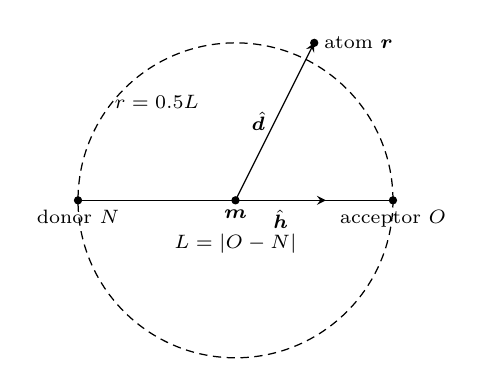
\begin{tikzpicture}[scale=1.0,line width=0.45pt,>=stealth]
  \coordinate (N) at (0,0);
  \coordinate (O) at (4.0,0);
  \coordinate (M) at (2.0,0);
  \coordinate (R) at (3.0,2.0);

  \draw (N) -- (O);
  \draw[->] (M) -- (3.15,0)
      node[midway,below] {\scriptsize \(\hat{\bm h}\)};
  \draw[->] (M) -- (R)
      node[midway,left] {\scriptsize \(\hat{\bm d}\)};
  \draw[densely dashed] (M) circle (2.0);

  \fill (N) circle (1.5pt) node[below] {\scriptsize donor \(N\)};
  \fill (O) circle (1.5pt) node[below] {\scriptsize acceptor \(O\)};
  \fill (M) circle (1.5pt) node[below] {\scriptsize \(\bm m\)};
  \fill (R) circle (1.5pt) node[right] {\scriptsize atom \(\bm r\)};
  \node at (2.0,-0.55) {\scriptsize \(L=|O-N|\)};
  \node at (1.0,1.25) {\scriptsize \(r=0.5L\)};
\end{tikzpicture}
\caption{The source is the \(N\cdots O\) segment reduced to its midpoint
\(\bm m\), length \(L\), and axis \(\hat{\bm h}\). The dashed circle marks the
per-atom near-field boundary \(r=0.5L\); the atom path accepts only outside it.}
\end{figure}

For an atom at \(\bm r_i\), the helper forms \code{d},
\(\bm d_{ik}=\bm r_i-\bm m_k\), its length \(r_{ik}\), the unit viewing
direction \(\hat{\bm d}_{ik}\), and the dot product
\(c_{ik}=\hat{\bm d}_{ik}\cdot\hat{\bm h}_k\). This is the McConnell helper
with \(\hat{\bm b}\) replaced by \(\hat{\bm h}\) and the expansion centre
replaced by the hydrogen-bond midpoint. If \(r_{ik}<\SI{0.1}{\angstrom}\), the
helper returns the zero-initialized result with \code{distance == 0}; it does
not clamp \(r\) to the guard distance.

\begin{codebox}
// Distilled from ComputeHBondKernel.
Vec3 d = atom_pos - hbond_midpoint;        // midpoint -> atom
double r = d.norm();
if (r < cfg("singularity_guard_distance")) return result;  // zero

result.distance = r;
double r3 = r * r * r;
Vec3 d_hat = d / r;
double c = d_hat.dot(h_hat);

result.f = (3.0 * c * c - 1.0) / r3;

for (int a = 0; a < 3; ++a)
    for (int b = 0; b < 3; ++b)
        result.M_over_r3(a,b) =
            (9.0*c*d_hat(a)*h_hat(b)
             -3.0*h_hat(a)*h_hat(b)
             -(3.0*d_hat(a)*d_hat(b) - (a == b ? 1.0 : 0.0))) / r3;
\end{codebox}

The scalar \code{f} is accumulated over the same accepted atom--source set as
the tensor. Its relationship to the trace of the asymmetric \(M\), and the way
the three terms populate \(T_0\), \(T_1\), and \(T_2\), are the same as in the
McConnell addendum after the substitution
\(\hat{\bm b}\mapsto\hat{\bm h}\).

\section{Filters and accumulation}

After the helper has produced a distance and candidate tensor, the atom path
builds the evaluation context consumed by the filters. The filter set is
minimum distance, self-source, then near-field. A rejected pair changes no
accumulator: not the tensor sum, not \code{f\_sum}, not the nearest-source
record, and not the \(\SI{3.5}{\angstrom}\) count.

\begin{codebox}
filters.Add(std::make_unique<MinDistanceFilter>());
filters.Add(std::make_unique<SelfSourceFilter>());
filters.Add(std::make_unique<DipolarNearFieldFilter>());

HBondKernelResult kernel =
    ComputeHBondKernel(atom_pos, hb.midpoint, hb.h_hat);

ctx.distance = kernel.distance;
ctx.source_extent = hb.distance;          // N...O length L
ctx.atom_index = ai;
ctx.source_atom_a = hb.donor_N;
ctx.source_atom_b = hb.acceptor_O;
ctx.sequence_separation = std::min(sep_to_donor, sep_to_acceptor);

if (!filters.AcceptAll(ctx)) continue;

if (kernel.distance < cfg("hbond_counting_radius")) ++nearby_count; // 3.5 A
if (kernel.distance < nearest_dist) { nearest_dist = kernel.distance; ... }

M_total += kernel.M_over_r3;
f_sum += kernel.f;
\end{codebox}

\code{MinDistanceFilter} requires \(r\ge\SI{0.1}{\angstrom}\). For a helper
return from below the guard, \code{kernel.distance} is zero and this filter
omits the pair. \code{SelfSourceFilter} rejects the exact donor \(N\) and
acceptor \(O\) atom indices. \code{DipolarNearFieldFilter} requires
\[
  r > \code{near\_field\_exclusion\_ratio}\,L = 0.5L .
\]
Equality at \(0.5L\) is rejected on the atom path. The
\code{sequence\_separation} field is filled with the nearest endpoint-residue
gap, but this filter set does not include \code{SequentialExclusionFilter};
sequence separation affects source resolution above, not later atom--source
evaluation.

There is no spatial search cutoff in this path. \code{SpatialIndexResult} is a
declared dependency, but after DSSP has supplied the source list the code loops
over every resolved hydrogen bond for every atom. The only atom--source
distance gates in the atom loop are the singularity and near-field filters;
otherwise the kernel keeps its \(r^{-3}\) dependence for distant accepted
terms. The count diagnostic
uses accepted pairs only and tests \(r<\SI{3.5}{\angstrom}\), so equality at
\(\SI{3.5}{\angstrom}\) is not counted.

\section{Sampling path and outputs}

\code{SampleKernelAt} evaluates the same stored source list at an arbitrary
point. Because that point has no atom index, this path has no donor/acceptor
self-source filter. It also uses an inline near-field test with a different
boundary from the atom filter: it skips \(r<0.5L\), so equality at \(0.5L\) is
kept.

\begin{codebox}
if (!conf_ || hbond_midpoints_.empty()) return SphericalTensor{};

Mat3 M_total = Mat3::Zero();
for (size_t hi = 0; hi < hbond_midpoints_.size(); ++hi) {
    auto kernel = ComputeHBondKernel(point, hbond_midpoints_[hi],
                                     hbond_directions_[hi]);
    if (kernel.distance < cfg("singularity_guard_distance")) continue;
    if (kernel.distance < cfg("near_field_exclusion_ratio") *
                          hbond_distances_[hi]) continue;

    M_total += kernel.M_over_r3;
}
return SphericalTensor::Decompose(M_total);
\end{codebox}

For atoms, the stored tensor output is the direct decomposition of the raw
asymmetric sum \(\bm M_i=\sum_k \bm M^{(ik)}\). There is no symmetrization and
no trace subtraction before \code{SphericalTensor::Decompose}. The nearest
source is tracked only among accepted pairs; a local \(\SI{99}{\angstrom}\)
sentinel initializes that search, but if no source is accepted the atom's
written nearest-distance and inverse-cube fields remain their zero defaults.

\begin{codebox}
if (nearest_hb_idx != SIZE_MAX) {
    ca.hbond_nearest_dist = nearest_dist;
    ca.hbond_nearest_dir =
        (atom_pos - nearest_hb.midpoint).normalized();
    ca.hbond_inv_d3 = 1.0 / (nearest_dist * nearest_dist * nearest_dist);

    auto nearest_kernel =
        ComputeHBondKernel(atom_pos, nearest_hb.midpoint, nearest_hb.h_hat);
    ca.hbond_nearest_spherical =
        SphericalTensor::Decompose(nearest_kernel.M_over_r3);
}

ca.hbond_shielding_contribution =
    SphericalTensor::Decompose(M_total);   // raw M, T0 + T1 + T2
ca.hbond_mcconnell_scalar = f_sum;
\end{codebox}

The writer emits two arrays. \code{hbond\_shielding.npy} is \((N,9)\) in the
shared packed order
\[
  [\,T_0,\;T_1[0..2],\;T_2[0..4]\,]
\]
written by \code{PackFull9}. It is the full asymmetric \(M\) decomposition.
\code{hbond\_scalars.npy} is \((N,4)\): nearest atom-to-midpoint distance, the
corresponding \(1/r^3\) field, accepted-source count with
\(r<\SI{3.5}{\angstrom}\), and the accepted \(\sum f\). HBond writes
no file analogous to McConnell's category \(T_2\) arrays. No HBond output first
takes the symmetric-traceless projection alone; the symmetric-traceless part is
present only as the \(T_2\) channel inside the full decomposition.

\begin{codebox}
ca.hbond_shielding_contribution.PackFull9(&shielding[i*9]);

scalars[i*4 + 0] = ca.hbond_nearest_dist;
scalars[i*4 + 1] = ca.hbond_inv_d3;
scalars[i*4 + 2] = double(ca.hbond_count_within_3_5A);
scalars[i*4 + 3] = ca.hbond_mcconnell_scalar;

WriteFloat64("hbond_shielding.npy", shielding.data(), N, 9);
WriteFloat64("hbond_scalars.npy", scalars.data(), N, 4);
\end{codebox}

\section{Glossary}

\textbf{DSSP partner slot.} One residue pointing at another it hydrogen-bonds to
(a per-residue DSSP field holding a partner residue index, with the actual \(N\)
and \(O\) atoms still to be looked up). If residue \(i\)
has acceptor slot \(j\), HBond turns it into \(N_i\to O_j\); if residue \(i\)
has donor slot \(j\), it turns it into \(N_j\to O_i\). Formally, each slot
contains a residue index or \code{SIZE\_MAX}, and HBond maps a valid slot to an
ordered backbone donor--acceptor atom pair.

\textbf{Hydrogen-bond source segment.} The source is the \(N\cdots O\) line
collapsed to a midpoint, a length, and an axis. A donor \(N\) at
\((0,0,0)\) and acceptor \(O\) at \((3,0,0)\) produce midpoint
\((1.5,0,0)\), length \(\SI{3}{\angstrom}\), and axis \((1,0,0)\). Formally,
\(\bm m=(\bm n+\bm o)/2\), \(L=|\bm o-\bm n|\), and
\(\hat{\bm h}=(\bm o-\bm n)/L\).

\textbf{Near-field exclusion.} A blind spot around the \(N\cdots O\) segment,
where the atom sits too close for the midpoint to stand in for the two-point
source (the atom path drops any atom whose distance to the midpoint is at or
below \(\rho_{\mathrm{nf}}L\), the ball of radius half the \(N\cdots O\) length
when \(\rho_{\mathrm{nf}}=0.5\)). For an \(N\cdots O\)
length of \(\SI{3}{\angstrom}\), the atom path omits an evaluation at
\(r=\SI{1.5}{\angstrom}\) and accepts one outside that distance. Formally, the
atom filter is \(r>\rho_{\mathrm{nf}}L\), with
\(\rho_{\mathrm{nf}}=\code{near\_field\_exclusion\_ratio}=0.5\).

\textbf{Spherical tensor split.} A \(3\times3\) tensor holds three kinds of
content that rotate without mixing --- an orientation-free size (the scalar
trace, \(T_0\)), an axial twist from its antisymmetric part (the three \(T_1\)
components), and a five-number traceless shape for the rest of the
direction-dependence (the five \(T_2\) components). In HBond,
\code{hbond\_shielding.npy} keeps all nine
numbers from the raw asymmetric McConnell-family sum, while no written HBond
array keeps only the symmetric-traceless projection. Formally, it is the
closed-form split of a \(3\times3\) tensor's nine components into dimensions
\(1+3+5\), with the \(T_2\) basis normalized to preserve the Frobenius norm.

\end{document}
